\documentclass[tikz]{standalone}

\begin{document}
    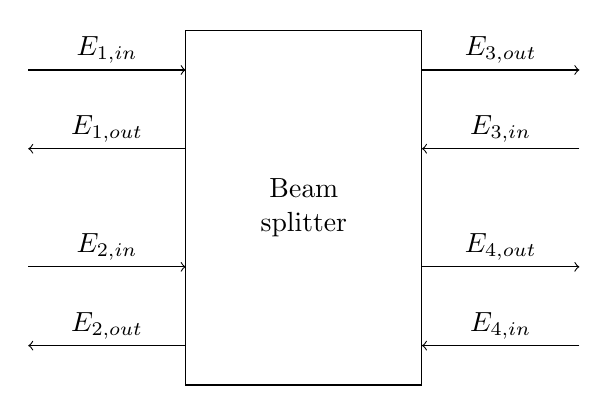
\begin{tikzpicture}
        \draw (0, 0) rectangle (3, 4.5);
        \node[text width=4cm, align=center] at (1.5, 2.25) {Beam\\splitter};

        \draw[->] (-2, 4) -- ++(2, 0) node(in1a){};
        \draw[->] (in1a) ++(0, -1) node(in1b){} -- ++(-2, 0);
        \draw (in1a) ++(-1, 0.25) node{$E_{1,\text{in}}$};
        \draw (in1b) ++(-1, 0.25) node{$E_{1,\text{out}}$};

        \draw[->] (in1b) ++(-2, -1.5) -- ++(2, 0) node(in2a){};
        \draw[->] (in2a) ++(0, -1) node(in2b){} -- ++(-2, 0);
        \draw (in2a) ++(-1, 0.25) node{$E_{2,\text{in}}$};
        \draw (in2b) ++(-1, 0.25) node{$E_{2,\text{out}}$};

        \draw[->] (in1a) ++(3, 0) node(out1a){} -- ++(2, 0);
        \draw[->] (in1b) ++(5, 0) -- ++(-2, 0) node(out1b){};
        \draw (out1a) ++(1, 0.25) node{$E_{3,\text{out}}$};
        \draw (out1b) ++(1, 0.25) node{$E_{3,\text{in}}$};

        \draw[->] (in2a) ++(3, 0) node(out2a){} -- ++(2, 0);
        \draw[->] (in2b) ++(5, 0) -- ++(-2, 0) node(out2b){};
        \draw (out2a) ++(1, 0.25) node{$E_{4,\text{out}}$};
        \draw (out2b) ++(1, 0.25) node{$E_{4,\text{in}}$};
    \end{tikzpicture}
\end{document}
